\chapter[Vícerozměrný regresní model \\ Testování hypotéz]{Vícerozměrný regresní model - testování hypotéz}

\section{Výběrové rozdělení OLS odhadů}

I při splnění všech Gauss-Markovových předpokladů může mít pravděpodobnostní rozdělení $\hat{\beta}_j$ v podstatě libovolný tvar. 
Lze dokázat, že pravděpodobnostní rozdělení $\hat{\beta}_j$ je závislé na pravděpodobnostním rozdělení chyb regresního modelu. 
Pro zjednodušení úvah o pravděpodobnostním rozdělení $\hat{\beta}_j$ předpokládejme, že pravděpodobnostní rozdělení chyb sleduje 
normální rozdělení; tento předpoklad nazýváme předpokladem normality.

\begin{assumption}[MLR.6 - normalita]
Chyba $u$ regresního modelu je nezávislá na vysvětlujících veličinách $x_1, x_2, ..., x_k$ a je normálně rozdělená s nulovou střední 
hodnotou a konstantním rozptylem $\sigma^2$, tj. $u \sim N(0, \sigma^2)$.

\raggedleft{$\clubsuit$}
\end{assumption}

\begin{figure}[htp]
\centering
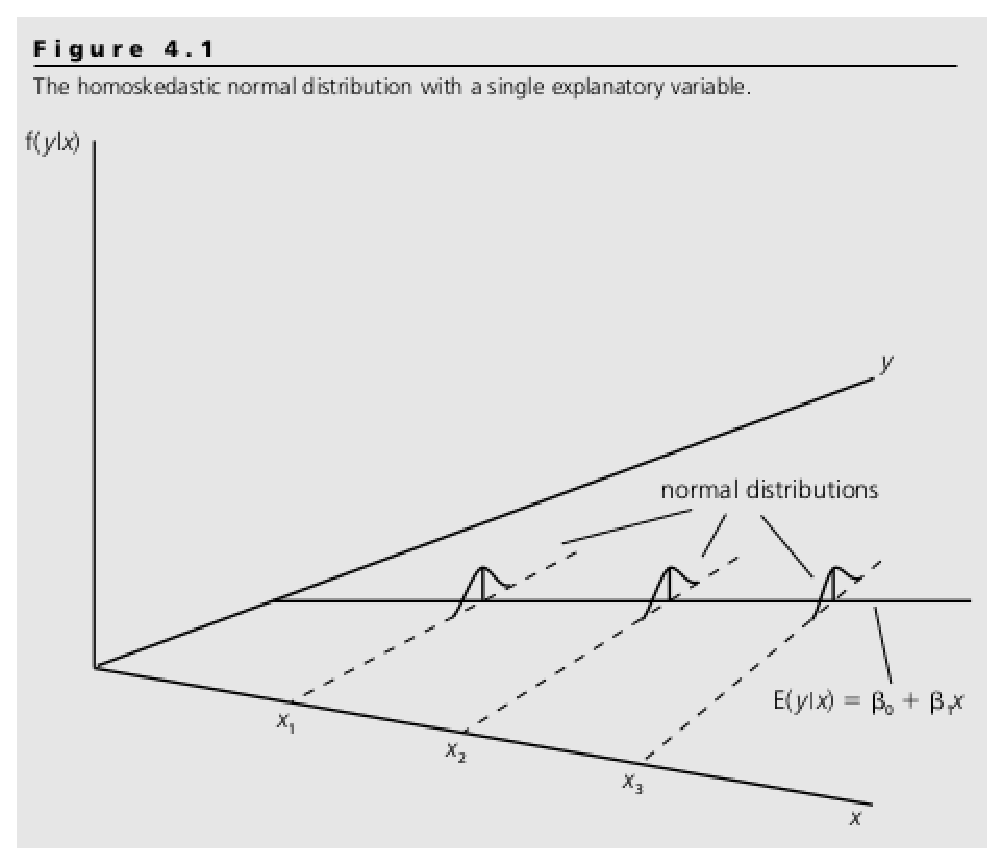
\includegraphics[scale = 0.5]{pictures/figure_4_1.eps}
\caption{Chyba $u$ jednoduchého regresního modelu, která sleduje normální rozdělení s nulovou střední hodnotou a konstantním rozptylem}
\label{figure_4_1}
\end{figure} 


Platnost předpokladu MLR.6 implikuje také platnost předpokladů MLR.4 a MLR.5. MLR.1 až MLR.6 jsou nazývány předpoklady klasického 
lineárního modelu (classical linear model (CLM) assumptions). Při splnění CLM předpokladů jsou OLS odhady $\hat{\beta}_0, 
\hat{\beta}_1, ..., \hat{\beta}_k$ efektivnějšími než by byly při splnění pouze Gauss-Markovových předpokladů. Lze dokázat, že tyto odhady 
jsou nestrannými odhady s minimálním rozptylem a to nejen mezi lineárními ale všemi typy odhadů.

Předpoklady klasického lineární modelu lze shrnout do rovnice
\begin{equation}
y|x_1, x_2, ..., x_k \sim N(\beta_0 + \beta_1 x_1 + \beta_2 x_2 + ... + \beta_k x_k).
\end{equation}
Protože chyba $u$ je součtem vlivu mnoha nejrůznějších faktorů ovlivňujících $y$, lze s odvoláním na centrální limitní větu 
předpokládat, že $u$ sleduje přibližně normální rozdělení. Hlavním problémem tohoto argumentu je implicitní předpoklad, že faktory, které 
vstupují do chyby $u$, jí ovlivňují odděleně a tudíž že tyto vlivy lze jednoduše sčítat. Pokud je $u$ komplikovanou funkcí těchto 
reziduálních faktorů, nemusí být tento předpoklad splněn. V některých případech lze problém předpokladu normality vyřešit, např. 
aplikací přirozeného logaritmu na vysvětlované popř. vysvětlující veličiny, která pravděpodobností rozdělení chyby $u$ normálnímu 
rozdělení přiblíží. Prozatím však jednoduše máme za to, že je předpoklad normality splněn.
\begin{theorem}[Normální výběrové rozdělení]
Pro odhad regresních parametrů na základě náhodného výběru při splnění CLM předpokladů MLR.1 až MLR.6 platí
\begin{equation}
\hat{\beta_j} \sim N(\beta_j, var[\hat{\beta}_j]),
\end{equation}
kde $var(\hat{\beta}_j)$ je dáno rovnicí (3.34). Proto $\frac{\hat{\beta}_j - \beta_j}{sd(\hat{\beta}_j)} \sim N(0, 1)$.

\raggedleft{$\clubsuit$}
\end{theorem}
Každé $\hat{\beta}_i$ lze zapsat ve tvaru $\hat{\beta}_j = \beta_j + \sum_{i = 1}^n w_{ij}u_i$, kde $w_{ij} = \frac{\hat{r}_{ij}}{SSR_j}$,
$\hat{r}_{ij}$ je $i$-té reziduum z regresního modelu $x_j$ na ostatní vysvětlující veličiny a $SSR_j$ je součtem čtverců reziduí této 
regrese. Protože $w_{ij}$ závisí pouze na nezávislých veličinách, lze s ní nakládat jako s nenáhodnou veličinou. $\hat{\beta}_j$ je tak lineární 
kombinací chyb $\{u_i: i = 1, 2, ..., n\}$ ve výběru. Vzhledem k předpokladu normality pak $\hat{\beta}_j$ sleduje normální rozdělení.

\section{Testování hypotézy jednoho parametru - $t$ test}
\begin{theorem}[$t$ rozdělení standardizovaných odhadů]
Při splnění CLM předpokladů MLR.1 až MLR.6 platí
\begin{equation}
\frac{\hat{\beta}_j - \beta}{se(\hat{\beta}_j)} \sim t_{n-k-1},
\end{equation}
kde $k + 1$ je počet odhadovaných parametrů regresního modelu $y = \beta_0 + \beta_1 x_1 + ... + \beta_k x_k + u$.

\raggedleft{$\clubsuit$}
\end{theorem}
$t$ rozdělení v (4.3) vychází ze skutečnosti, že konstanta $\sigma$ v $se(\hat{\beta}_j)$ byla nahrazena náhodnou veličinou $\hat{\sigma}$. 
Výše uvedená věta je extrémně důležitá, protože nám umožňuje testovat hypotézy týkající se parametru $\beta_j$. Pro účely 
testování hypotéz je pak definována tzv. $t$ statistika
\begin{equation}
t_{\hat{\beta}_j} \equiv \frac{\hat{\beta}_j}{se(\hat{\beta}_j)}.
\end{equation}

\subsection{Jednostranný test}

V rámci jednostranného testu zjišťujeme, zda-li je hodnota parametru $\beta_j$ menší či větší než určitá konstanta $c$. Nejčastěji se testuje 
$\beta_j$ proti $c = 0$, což znamená, že nulová a alternativní hypotéza mají podobu
\begin{equation}
H_0: \beta_j \le 0 ~~~~~~ H_1: \beta_j > 0,
\end{equation}
popř.
\begin{equation}
H_0: \beta_j \ge 0 ~~~~~~ H_1: \beta_j < 0.
\end{equation}
V prvním případě testujeme, zda-li je $\beta_j < 0$, kdežto ve druhém případě zda-li je $\beta_j > 0$. V prvním případě nulovou 
hypotézu zamítneme, pokud odpovídající $t$ statistika $t_{\beta_j} = \frac{\hat{\beta}_j}{se(\hat{\beta}_j)}$ splňuje podmínku
\begin{equation}
t_{\beta_j} > t_{n-k-1}^{1 - \alpha}
\end{equation}
a druhém případě, pokud splňuje podmínku
\begin{equation}
t_{\beta_j} < t_{n-k-1}^{\alpha},
\end{equation}
kde $t_{n-k-1}^{\alpha}$ představuje $\alpha$ kvantil Studentova rozdělení s $n-k-1$ stupni volnosti. Kvantil $\alpha$ též nazýváme hladinou významnosti.

\begin{figure}[htp]
\centering
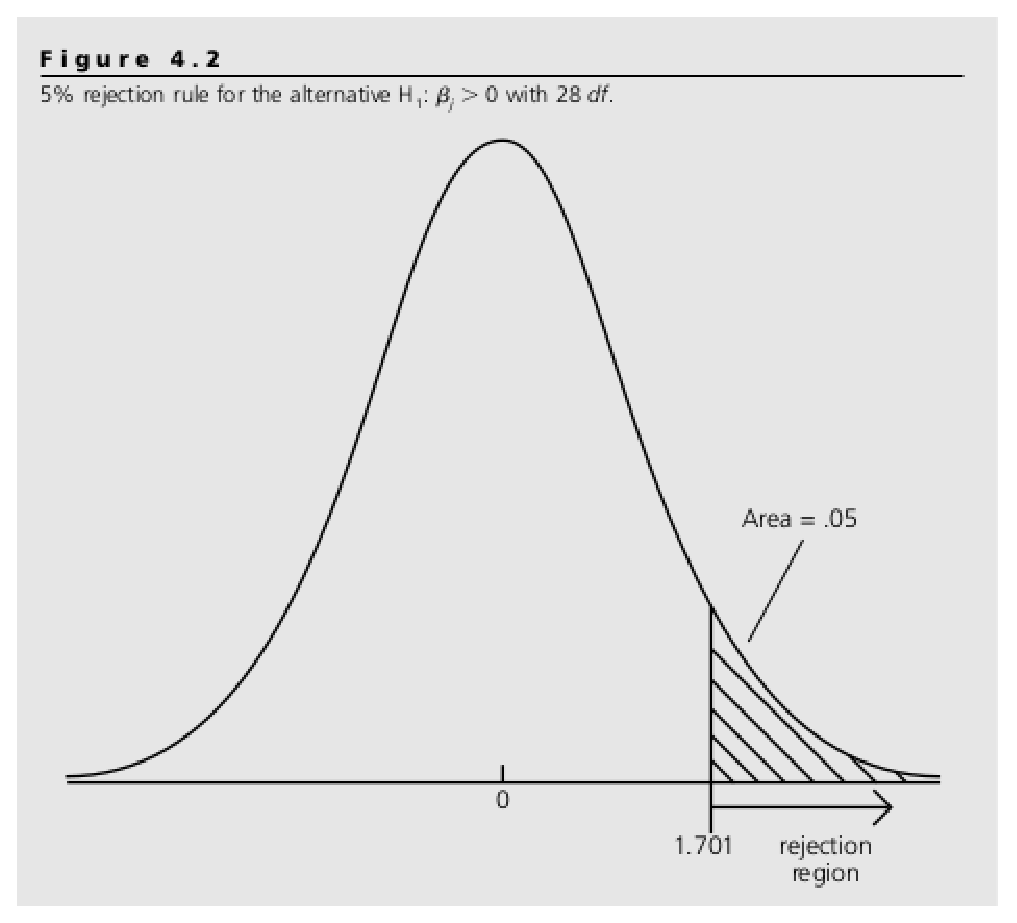
\includegraphics[scale = 0.5]{pictures/figure_4_2.eps}
\caption{Jednostranný test s alternativní hypotézou $H_1: \beta_j > 0$}
\label{figure_4_2}
\end{figure}

\begin{figure}[htp]
\centering
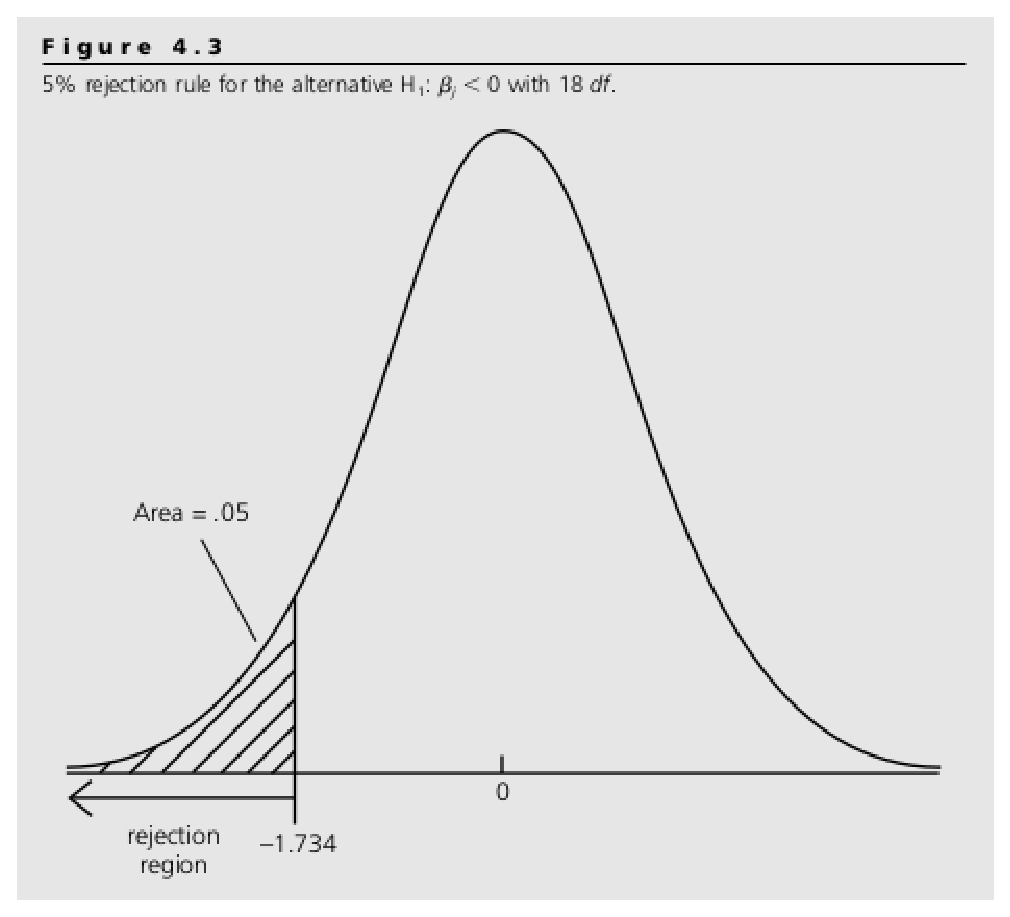
\includegraphics[scale = 0.5]{pictures/figure_4_3.eps}
\caption{Jednostranný test s alternativní hypotézou $H_1: \beta_j < 0$}
\label{figure_4_3}
\end{figure} 

Pokud je $c \ne 0$, pak se nulová a alternativní hypotéza změní na $H_0: \beta_j \le c, H_1: \beta_j > c$ popř. na $H_0: \beta_j \ge c, H_1: \beta_j < c$. Nulovou hypotézu zamítneme, pokud $t_{\beta_j} < t_{n-k-1}^{\alpha}$ popř. $t_{\beta_j} > t_{n-k-1}^{1 - \alpha}$, kde $t_{\beta_j} = \frac{\hat{\beta}_j - c}{se(\hat{\beta}_j)}$.

\subsection{Dvoustranný test}

V případě dvoustranného testu přejde nulová a alternativní hypotéza do tvaru
\begin{equation}
H_0: \beta_j = 0 ~~~~~~ H_1: \beta_j \ne 0,
\end{equation}
kdy nulovou hypotézu zamítneme pokud
\begin{equation}
|t_{\beta_j}| > t_{n-k-1}^{1 - \frac{\alpha}{2}}.
\end{equation}
Na rozdíl od jednostranného testu, který existuje ve dvou podobách, máme pouze jednu formu dvoustranného testu. V rámci nulové hypotézy pak testujeme, zda-li je $\beta_j$ rovno nule.

\begin{figure}[htp]
\centering
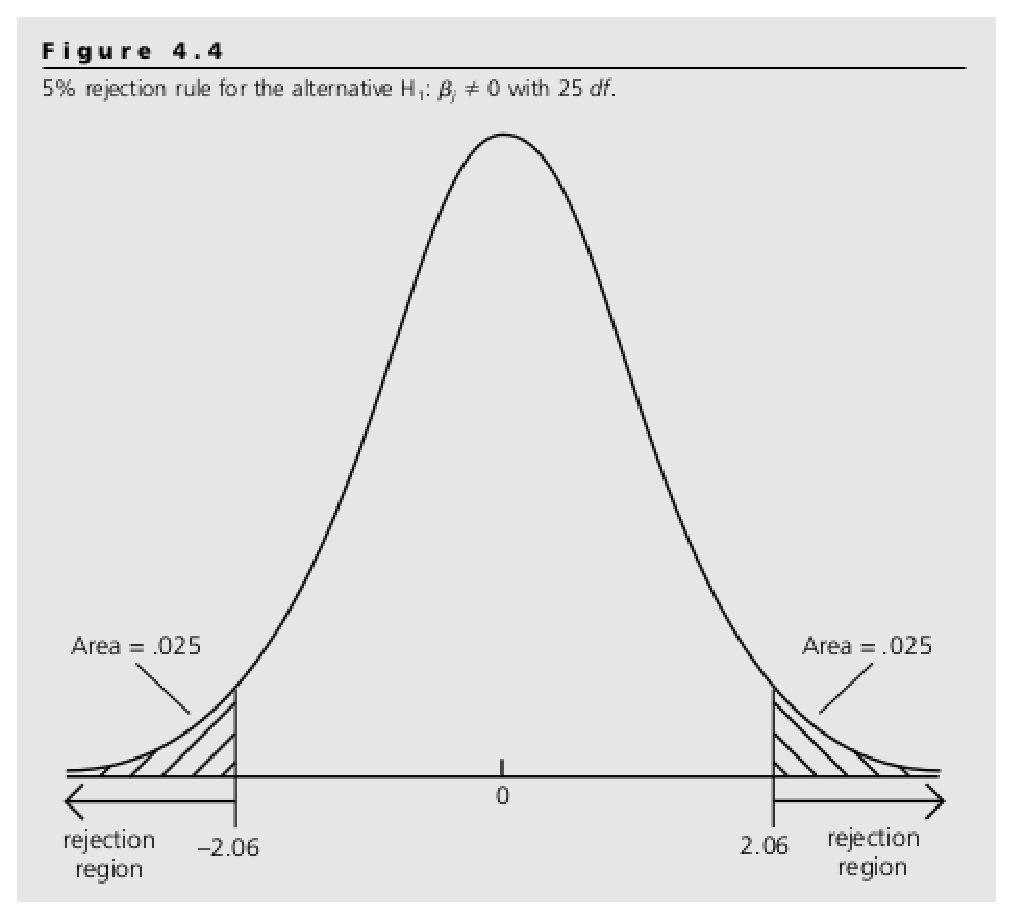
\includegraphics[scale = 0.5]{pictures/figure_4_4.eps}
\caption{Dvoustranný test s alternativní hypotézou $H_1: \beta_j \ne 0$}
\label{figure_4_4}
\end{figure} 

Podobně jako v případě jednostranného testu lze dvoustranný test snadno zobecnit na případy, kdy $c \ne 0$. V tomto případě nulová a alternativní hypotéza přejde na $H_0: \beta_j = c, H_1: \beta_j \ne c$, kdy nulovou hypotézu zamítneme, pokud $|t_{\beta_j}| > t_{n-k-1}^{1 - \frac{\alpha}{2}}$, kde $t_{\beta_j} = \frac{\hat{\beta}_j - c}{se(\hat{\beta}_j)}$.

\subsection{p-hodnota (p-value)}

Při testování hypotéz je třeba zvolit hladinu významnosti $\alpha$. Je třeba zdůraznit, že neexistuje žádná ``správná'' hladina 
významnosti. Nicméně pro danou hodnotu $t$ statistiky si můžeme položit otázku, jaká je nejnižší hladina významnosti, pro kterou je 
nulová hypotéza zamítnuta. Tuto hladinu významnosti nazýváme p-hodnotou. Z této definice je zřejmé, že nízká p-hodnota je argumentem pro 
zamítnutí nulové hypotézy, zatímco vysoká p-hodnota je argumentem pro přijetí nulové hypotézy. Jinými slovy, je-li námi zvolená 
hladina významnosti rovna $\alpha$, pak pro $p-hodnota < \alpha$ nulovou hypotézu zamítneme.

\subsection{Interval spolehlivosti}

V řadě případů je žádoucí zjistit interval, ve kterém se parametr $\beta_j$ s určitou pravděpodobností nachází. S ohledem na větu (4.2) víme, že
\begin{equation}
\frac{\hat{\beta}_j - \beta}{se(\hat{\beta}_j)} \sim t_{n - k -1}.
\end{equation}
Pokud tedy chceme najít interval, ve kterém se s pravděpodobností $1 - \alpha$ bude nacházet parametr $\beta$, pak prostou modifikací výše 
uvedeného získáme
\begin{equation}
\hat{\beta}_j - t_{n - k -1}^{1 - \frac{\alpha}{2}} \le \beta \le \hat{\beta}_j + t_{n - k -1}^{1 - \frac{\alpha}{2}}.
\end{equation}
Pokud zkombinujeme (4.10) s (4.11) a výsledek porovnáme s (4.12), je zřejmé, že interval spolehlivosti a dvoustranný $t$ test jsou postaveny na 
stejném logickém základě.

\subsection{Testování hypotéz zahrnujících lineární kombinaci vícero parametrů}

Uvažujme jednoduchý regresní model, ve kterém provádíme regresi logaritmu příjmu na počet roků strávených na bakalářském a magisterském 
studijním oboru a počtu roků praxe, tj.
\begin{equation}
ln(wage) = \beta_0 + \beta_1 bac + \beta_2 mag + \beta_3 exp + u.
\end{equation}
Předpokládejme, že chceme testovat $H_0: \beta_1 = \beta_2$ proti $H_1: \beta_1 < \beta_2$, tj. zda-li jeden rok studia bakalářského oboru 
zvýší mzdu o stejné procento jako rok studia magisterského oboru. Nulovou a alternativní hypotézu lze přepsat do tvaru $H_0: \beta_1 - 
\beta_2 = 0$ a $H_1: \beta_1 - \beta_2 < 0$. To znamená, že namísto jednoho parametru, testujeme lineární kombinaci dvou parametrů. Je 
důležité si uvědomit, že pravděpodobnostní rozdělení odhadu každého z parametrů sleduje při splnění CLM předpokladů Studentovo 
rozdělení stejně jako každá jejich lineární kombinace. Proto jsme pro $\hat{\theta} = \hat{\beta}_1 - \hat{\beta}_2$ teoreticky schopni zkonstruovat $t$ statistiku
\begin{equation}
t = \frac{\hat{\theta} - \theta}{se(\hat{\theta})},
\end{equation}
kde $se(\hat{\theta}) = \sqrt{var[\hat{\beta}_1] + var[\hat{\beta}_1] - 2cov[\hat{\beta}_1, \hat{\beta}_2]}$ a tu následně použít pro účely 
testování nulové hypotézy. V praxi bohužel tento postup naráží na neznalost $cov[\hat{\beta}_1, \hat{\beta}_2]$. Tento problém však lze 
relativně snadno obejít přeformulováním původního regresního modelu do tvaru
\begin{equation}
ln(wage) = \beta_0 + \theta bac + \beta_2 (bac + mag) + \beta_3 exp + u.
\end{equation}
Po této upravě provedeme odhad modelu pomocí OLS a následně aplikujeme standardní dvoustranný $t$ test na parametr $\theta$, kde testujeme 
$H_0: \theta = 0$ proti $H_1: \theta \ne 0$.

Analogický postup lze použít také v případech jiných lineárních kombinací, např. při 
testování nulové hypotézy $H_0: \beta_1 = 0.75 \beta_2$ proti alternativní hypotéze $H_1: \beta_1 \ne 0.75 \beta_2$. Kromě dvoustranných 
hypotéz lze testovat také jednostranné hypotézy.

\section{Testování vícero lineárních omezení - $F$ test}

\subsection{Testování významnosti vícero parametrů}

Předpokládejme, že chceme testovat, zda-li má určitá skupina vysvětlujících veličin vliv na vysvětlovanou veličinu. Uvažujme 
vícerozměrný regresní model
\begin{equation}
y = \beta_0 + \beta_1 x_1 + \beta_2 x_2 + \beta_3 x_3 + \beta_4 x_4 + \beta_5 x_5 + u,
\end{equation}
pro který budeme testovat nulovou hypotézu
\begin{equation}
H_0: \beta_3 = 0, \beta_4 = 0, \beta_5 = 0.
\end{equation}
Hypotézu v tomto tvaru nazýváme vícenásobnou 
popř. sdruženou hypotézou. Alternativní hypotéza $H_1: \textit{nepravdivá} ~~ H_0$ je platná, pokud alespoň jeden parametr z $\beta_3$, $\beta_4$ nebo 
$\beta_5$ je různý od nuly.

Na první pohled by se mohlo zdát, že (4.17) můžeme testovat parametr po parametru s využitím klasického dvoustranného $t$ testu. Nicméně 
jednotlivé $t$ testy se zaměřují vždy jen na ``svůj'' parametr. Pokud bychom tedy hypotézu (4.17) testovali pomocí série $t$ testů, byli bychom příliš 
konzervativní. Intuitivně lze odhadnout, že sdružený test by mohl být založen na změně $R^2$. Z předchozího textu víme, že 
přidáním vysvětlujících veličin se zvýší $R^2$ modelu. Otázkou tedy je, zda-li je toto zvýšení dostatečné na to, aby přidání 
těchto vysvětlujících veličin ospravedlnilo.

Uvažujme regresní model
\begin{equation}
y = \beta_0 + \beta_1 x_1 + ... + \beta_k x_k + u.
\end{equation}
Pro účely následujícího textu budeme tento model označovat jako neomezený (unrestricted model). Uvažujme nulovou hypotézu
\begin{equation}
H_0: \beta_{k - q + 1} = 0, ..., \beta_k = 0.
\end{equation}
Pokud z původního neomezeného modelu vypustíme vysvětlující veličiny $\beta_{k - q + 1}, ..., \beta_k$, získáme tzv. omezený model 
(restricted model) ve tvaru
\begin{equation}
y = \beta_0 + \beta_1 x_1 + ... + \beta_{k - q}x_{k - q} + u.
\end{equation}
Definujme tzv. $F$ statistiku
\begin{equation}
F \equiv \frac{\frac{SSR_r - SSR_{ur}}{q}}{\frac{SSR_{ur}}{n - k - 1}},
\end{equation}
kde $SSR_r$ je reziduální součet čtverců omezeného modelu, $SSR_{ur}$ je reziduální součet čtverců neomezeného modelu a $q$ představuje 
rozdíl stupňů volnosti mezi neomezeným a omezeným modelem (což odpovídá počtu testovaných parametrů), tj. $q = df_{ur} - df_{r}$. Připomeňme, že 
$R^2 = 1 - \frac{SSR}{SST}$, kde $SSR = \sum_{i = 1}^n \hat{u}_i^2$ a $SST = \sum_{i = 1}^n (y_i - \overline{y})^2$.

$F$ statistika sleduje $F$ rozdělení s $(q, n - k - 1)$ stupni volnosti, tj.
\begin{equation}
F \sim F_{q, n - k - 1}.
\end{equation}
Nulovou hypotézu tedy zamítneme ve prospěch alternativní hypotézy, pokud
\begin{equation}
F > F_{q, n - k - 1}^{\alpha},
\end{equation}
kde $\alpha$ představuje námi zvolenou hladinu významnosti. Pokud je nulová hypotéza zamítnuta, říkáme, že vysvětlující veličiny $x_{k 
- q + 1, ..., x_k}$ jsou sdruženě statisticky významné. V praxi se může stát, že ačkoliv jsou jednotlivé vysvětlující veličiny 
individuálně statisticky nevýznamné, jsou sdruženě statisticky významné. Poněkud překvapivě však může nastat i opačná situace, tj. 
pokud ke skupině statisticky nevýznamných veličin přidáme jednu statisticky významnou, můžeme dojít k závěru, že skupina těchto 
vysvětlujících veličin je jako celek sdruženě statisticky nevýznamná.

\subsection{Vztah mezi $F$ a $t$ testem}

Lze dokázat, že $F$ statistika pro testování jednoho parametru je rovna čtverci odpovídající $t$ statistiky. Protože $t_{n - k - 1}^2$ a 
$F_{1, n - k - 1}$ sledují stejné pravděpodobnostní rozdělení, vedou obě statistiky v případě dvoustranného testu k shodným závěrům.

\subsection{$R^2$ forma $F$ statistiky}

Připomeňme, že $SSR_r = SST(1 - R_r^2)$ a $SSR_{ur} = SST(1 - R_{ur}^2)$. Dosazením do (4.21) získáme tzv. $R^2$ formu $F$ statistiky.
\begin{equation}
F = \frac{\frac{R_{ur}^2 - R_t^2}{q}}{\frac{(1 - R_{ur}^2)}{n - k -1}} = \frac{\frac{R_{ur}^2 - R_r^2}{q}}{\frac{(1 - R_{ur}^2)}{n - k - 1}}
\end{equation}

\subsection{Výpočet p-hodnoty $F$ testu}

P-hodnotu $F$ testu definujeme jako
\begin{equation}
p-hodnota = P(\mathcal{F} > F),
\end{equation}
kde $\mathcal{F}$ představuje náhodnou veličinu z $F$ rozdělení s $(q, n - k - 1)$ stupni volnosti a $F$ je hodnota $F$ statistiky. P-hodnota pak 
představuje pravděpodobnost, že budeme pozorovat danou hodnotu $F$ statistiky za předpokladu platnosti nulové hypotézy. Pokud je p-hodnota 
nižší než námi zvolená hladina významnosti $\alpha$, nulovou hypotézu zamítneme.

\subsection{Test celkové statistické významnosti regresního modelu}

Uvažujme regresní model (4.18), nulovou hypotézu
\begin{equation}
H_0: \beta_1 = \beta_2 = ... = \beta_k = 0
\end{equation}
a alternativní hypotézu, která říká, že alespoň jeden parametr $\beta_j$ je různý od nuly. Tento test nazýváme testem celkové 
statistické významnosti regresního modelu. Logika testu je stejná jako v případě klasického $F$ testu s tím, že omezený model má tvar
\begin{equation}
y = \beta_0 + u.
\end{equation}
Protože $R^2$ regresního modelu (4.27) je rovno nule, zjednoduší se $F$ statistika do tvaru
\begin{equation}
F = \frac{\frac{R^2}{k}}{\frac{1 - R^2}{n - k - 1}}
\end{equation}

\subsection{Testování obecných lineárních omezení}

Uvažujme regresní model
\begin{equation}
y = \beta_0 + \beta_1 x_1 + \beta_2 x_2 + \beta_3 x_3 + \beta_4 x_4 + u
\end{equation}
a nulovou hypotézu
\begin{equation}
H_0: \beta_1 = 1, \beta_2 = 0, \beta_3 = 0, \beta_4 = 0.
\end{equation}
Omezený model získáme dosazením omezení z nulové hypotézy do původního modelu. Omezený model má pak v našem konkrétním případě tvar
\begin{equation}
y - x_1 = \beta_0 + u.
\end{equation}
Pro účely výpočtu $F$ statistiky nemůžeme používat (4.24), protože závislá veličina v modelu (4.31) není $y$ ale $y - x_1$. Proto je 
třeba použít (4.31).
